\documentclass[article,12pt]{elsarticle}
\usepackage[spanish]{babel}
\usepackage[utf8]{inputenc}
\usepackage{amssymb}
\usepackage{flushend}
\usepackage{float}
\usepackage{anysize}
\usepackage{amsmath}
\usepackage{amsfonts}
\usepackage{dcolumn}
\usepackage{amsthm}
\usepackage{caption}
\usepackage{float}
\usepackage{subfigure}
\usepackage{graphicx}
\usepackage{lmodern}
\usepackage{booktabs}
\usepackage{color}
\usepackage{longtable}
\usepackage{rotating}
\usepackage{etoolbox}
\usepackage{comment}
\usepackage{pdflscape}
\usepackage{booktabs}


\begin{document}

\begin{frontmatter}
    \title{Laboratorio de Electromagnetismo \\  Práctica  4\\ 
        Flujo de electrones}
    \author{Iván Bautista Alvarado$^1$ y Andrés López González$^1$} %Aquí va el nombre de los integrantes que participaron en el informe.
    \address{$^1$ Facultad de Ciencias, Universidad Nacional Autónoma de México, M\'exico CDMX.}


    \begin{abstract}
     This study experimentally determined the electrical resistivity of nichrome using two complementary methodologies: direct measurement of resistance in different lengths of wire and obtaining the voltage-current characteristic curve. The results obtained through both methods showed excellent consistency, allowing the calculation of an average resistivity value of $(10.3 \pm 0.5) \cdot 10^{-8} \Omega m$ for the first method and $(10.7 \pm 0.5) \cdot 10^{-8} \Omega m$ for the second one. This value is within the range reported in the literature for nichrome, considering the variations attributable to the purity of the material and experimental conditions. The linear relationship observed between voltage and current confirms the validity of Ohm's law for nichrome in the studied range of values. The main sources of uncertainty in the experiment were analyzed, including errors in the measurement of length, diameter, voltage, and current. The results of this study contribute to a better understanding of the electrical properties of nichrome and have important implications for its application in various electronic devices.
    \end{abstract}

    \begin{keyword}
     Nichrome resistivity
Electrical conductivity
Voltage-current characteristics
Experimental determination
Material properties
    \end{keyword}
\end{frontmatter}

\section*{Resumen}
En este estudio se determinó experimentalmente la resistividad eléctrica del nicromel empleando dos metodologías complementarias: la medición directa de la resistencia en diferentes longitudes de alambre y la obtención de la curva característica voltaje-corriente. Los resultados obtenidos a través de ambos métodos mostraron una excelente consistencia, permitiendo calcular un valor promedio de resistividad de $(10.3 \pm 0.5) \cdot 10^{-8} \Omega m$ para el primer método y $(10.7 \pm 0.5) \cdot 10^{-8} \Omega m$ para el segundo. Este valor se encuentra dentro del rango reportado en la literatura para el nicromel, considerando las variaciones atribuibles a la pureza del material y las condiciones experimentales. La relación lineal observada entre el voltaje y la corriente confirma la validez de la ley de Ohm para el nicromel en el rango de valores estudiados. Las principales fuentes de incertidumbre en el experimento fueron analizadas, incluyendo los errores en las mediciones de longitud, diámetro, voltaje y corriente. Los resultados de este estudio contribuyen a una mejor comprensión de las propiedades eléctricas del nicromel y tienen implicaciones importantes para su aplicación en diversos dispositivos electrónicos.

\noindent \textit{Palabras Clave}: \textit{Palabras Clave}: Resistividad del nicromel, Conductividad eléctrica, Características voltaje-corriente, Determinación experimental, Propiedades de los materiales.\\ \hline

\section{Introducción}
    Uno de los descubrimientos importantes en la electrodinámica es la Ley de Ohm:
     \begin{equation}
        I = \frac{V}{R}
    \end{equation}
    Que nos dice que la corriente I que circula por un hilo es directamente proporcional a la diferencia de potencial V de sus extremos, pero inversamente proporcional a una cantidad R llamada resistencia. 
    La resistencia es una propiedad extensiva de los materiales, que indica qué tan difícil es pasar un flujo de electrones a través del material. Suponiendo que el flujo tiene una dirección paralela al campo eléctrico que los hace moverese, y considerando el área de la sección transversal del material, y su longitud. Tenemos que:
    \begin{equation}
        R = \rho  \frac{l}{A}
    \end{equation}
    En donde A es el área de la sección transversal y l la longitud del material.
    Al término $\rho$ se le llama resistividad, y esta es una propiedad intensiva del material. La resistividad también nos india qué tan difícil es hacer pasar un flujo, pero que únicamente depende del material, es decir, de su estructura molecular.
    Despejando de la ec. 2 podemos ver que
    \begin{equation}
        \rho = R  \frac{A}{l}
    \end{equation} 
    Es importante diferenciar la resistencia de la resistividad. Su diferencia más importante es que la resistencia es una propiedad intensiva y la resistividad es extensiva. Y por otro lado, la resistencia se mide en ohmios $[\Omega]$ y la resistividad en ohmios por metro $[\Omega \cdot m]$. \\

    Para medida de la resistividad en función del voltaje e intensidad, se puede mantener la longitud y área transversal constante según el experimento lo requiera, la ecuación 3 se convierte en lo siguiente:
    \begin{equation}
        \rho = \frac{V}{I}  \frac{A_i}{l_i} = \alpha_i \frac{V}{I}
    \end{equation} 
    \subsection{Hipótesis}
    Creemos que la resistencia va a cambiar dependiendo del grosor y de la longitud. Entre más grueso sea, mayor va a ser su resistencia, y entre más largo sea, de igual manera aumentará su resistencia. Estos cambios tendrán un comportamiento lineal.
    \subsection{Objetivos}
    Determinar las resistividades de los alambres de nicromel a partir de sus resistencias.
\section{Desarrollo Experimental / Métodos}
    Materiales utilizados:
    \begin{itemize}
        \item 1 Guitarrón
        \item 1 Flexómetro
        \item 1 Multímetro
        \item 1 Tornillo micrométrico
        \item 2 Pinzas caiman
        \item 4 Cables banana-banana
        \item 1 Fuente de poder (de voltaje)
    \end{itemize}
    ¨Primero se le ajustaron las cuerdas al guitarrón para que estuvieran tensas, y con el flexómetro se marcaron las distancias cada 10cm hasta el primer metro, midiendo desde las clavijas. Y con el tornillo micrométrico se midieron los diámetros de los alambres del guitarrón. 
    Después con el multímetro se midieron las resistencias. Se conectó un cable banana-banana al multímetro, y con un caimán en uno de los extremos se agarró a la clavija correspondiente al cable al que se le quería medir la resistencia, en la otra entrada del multímetro (para resistencias) se conectó el cable con la punta de prueba. Entonces, cada 10cm (las mediciones ya hechas) se colococó la punta de prueba y se anotó la resistencia registrada en el multímetro, repitiendo esto hasta el primer metro.
    Esto se hizo para 4 cuerdas del guitarrón. \\
    Después, se conectó la fuente de poder a una cuerda del guitarrón. Con un cable banana-banana conectado a la fuente de poder, se agarró con un caiman a la clavija correspondiente. y de la otra entrada se conectó con un cable banana-banana la entrada de la fuente al multímetro, que nos iba a medir el amperaje (intensidad de corriente) y desde el multímetro, fue conectado con un cable banana-banana, y un caiman al alambre, a la distancia a la que queríamos medir la resistencia para que de esta manera si pase la corriente por el alambre. Por último, usando otro multímetro, conectado a otro par de cables banana-banana y un caiman, se midió el voltaje que generaba la fuente en el alámbre.
    Ya teniendo el arreglo, se fue varió el amperaje que se suministraba con una distancia fija de 20cm, haciendo 10 mediciones distintas por cada alámbre. Y finalmente se repitió el proceso pero a una distancia de 40cm.
\section{Resultados y discusión}
    Para la primera parte, se obtuvo la siguiente tabla:
    \begin{table}[H]
\begin{tabular}{|c|c|c|c|c|}
\hline
\multicolumn{1}{|l|}{Distancia} & \multicolumn{1}{l|}{Primera Cuerda} & \multicolumn{1}{l|}{Segunda Cuerda} & \multicolumn{1}{l|}{Tercera Cuerda} & \multicolumn{1}{l|}{Cuarta Cuerda} \\ \hline
0.100$\pm$0.0005 m                                                     & 0.3                                 & 0.7                                 & 2.5                                 & 21.1                               \\ \hline
0.200$\pm$0.0005 m                                                    & 0.5                                 & 1.6                                 & 4.5                                 & 44.3                               \\ \hline
0.300$\pm$0.0005 m                                                    & 0.8                                 & 2.1                                 & 8.0                                   & 68.6                               \\ \hline
0.400$\pm$0.0005 m                                                   & 1.0                                   & 2.7                                 & 8.9                                 & 88.9                               \\ \hline
0.500$\pm$0.0005 m                                                  & 1.4                                 & 3.2                                 & 10.8                                & 109.5                              \\ \hline
0.600$\pm$0.0005 m                                                   & 1.6                                 & 3.7                                 & 12.8                                & 131.4                              \\ \hline
0.700$\pm$0.0005 m                                                    & 1.6                                 & 4.3                                 & 15.0                                  & 155.1                              \\ \hline
0.800$\pm$0.0005 m                                                  & 1.7                                 & 4.5                                 & 17.0                                  & 176.3                              \\ \hline
0.900$\pm$0.0005 m                                                  & 2.0                                  & 4.7                                 & 19.0                                  & 199.1                              \\ \hline
1.000$\pm$0.0005 m                                                 & 2.2                                 & 5.4                                 & 21.1                                & 221.1                              \\ \hline
\end{tabular}
\caption{Tabla de las resistencias medidas por cada 10cm en alambres de Nicromel de distinto grosor}
\end{table}
Al graficar estos datos, en una gráfica A/l vs R obtenemos un comportamiento lineal en la que teóricamente la pendiente corresponde a la resistividad. Vease la continuación la gráfica referente a la primera cuerda: %hacer gráfica$

\begin{figure}[h]
    \centering
    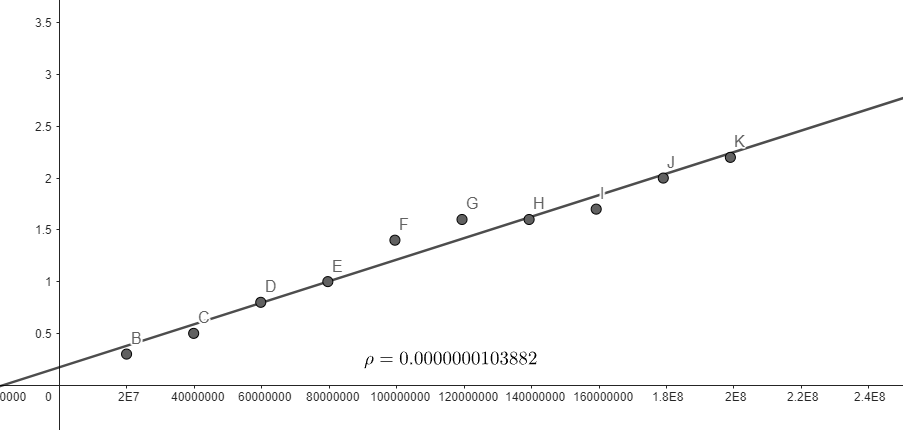
\includegraphics[width=1\linewidth]{R.png}
    \caption{Gráfica para la primer cuerda}
    \label{fig:enter-label}
\end{figure}

En la que la pendiente es la resistividad del material; para este caso de la primera cuerda hemos obtenido $\rho=0.0000000103882 \, \Omega m$. Para la segunda cuerda empleando el mismo método obtenemos la siguiente gráfica y en consecuencia la siguiente resistividad.

\newpage

\begin{figure}[h]
    \centering
    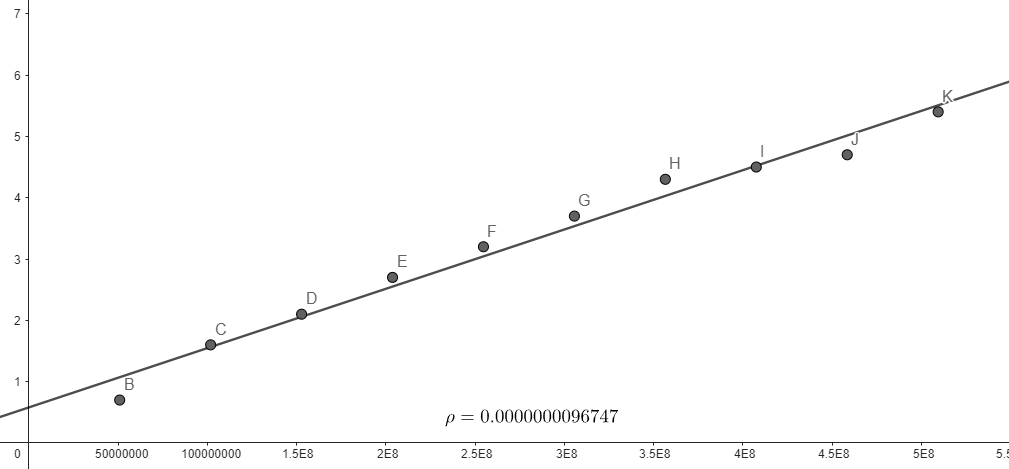
\includegraphics[width=0.75\linewidth]{Gráfica para la segunda cuerda.png}
    \caption{Gráfica para la segunda cuerda}
    \label{fig:enter-label}
\end{figure}\\

En donde la resistividad se ha mostrado demasiado similar, que por hipótesis es lo esperado pues esta es fija en cada material. Obtenemos que en este caso $\rho=0.0000000096747 \, \Omega m$; a continuación se muestra el gráfico para la tercera cuerda.\\

\begin{figure}[h]
    \centering
    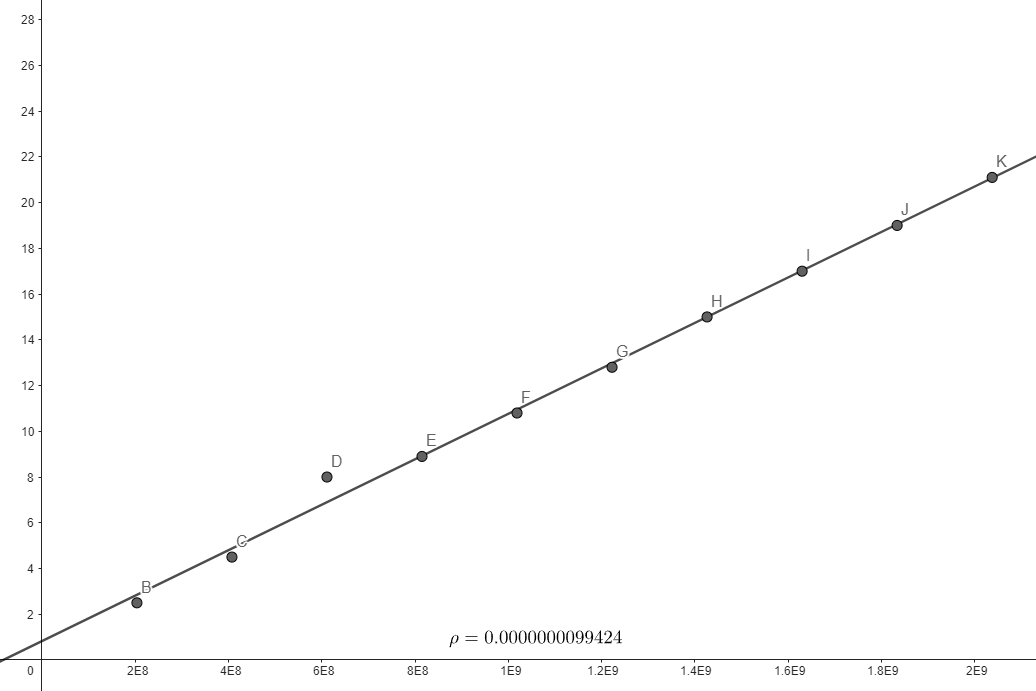
\includegraphics[width=0.75\linewidth]{Gráfica para la tercera cuerda.png}
    \caption{Gráfica para la tercera cuerda}
    \label{fig:enter-label}
\end{figure}\\

En donde la resistividad nuavemente apreciamos un valor excesivamente fiel, siendo esta $\rho=0.0000000099424 \, \Omega m$. Finalmente para nuestra última cuerda se obtiene.

\begin{figure}[h]
    \centering
    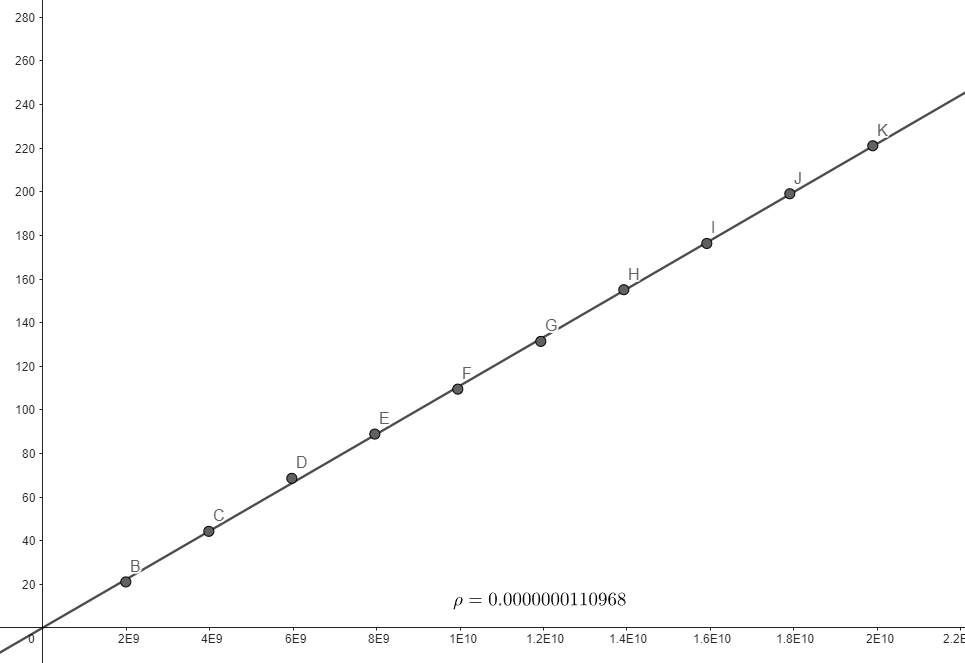
\includegraphics[width=0.75\linewidth]{Gráfica para la cuarta cuerda.png}
    \caption{Gráfica para la cuarta cuerda}
    \label{fig:enter-label}
\end{figure}

Con una resistividad de $\rho = 0.0000000110968 \Omega m$; para no acarrear incertidumbres he realizado la regresión lineal para un solo sistema con todos estos puntos, en los que se ha obtenido que el valor para la resistividad del nicromel es de $(10.3 \pm 0.5)\cdot 10^{-8} \, \Omega m$




\newpage

Para la segunda parte, se obtuvo una numero cantidad de tablas, por lo que omitiré la parte de adjuntar el gráfico para no saturar esta sección pero he ocupado exactamente el mismo método pero ahora con una gráfica voltaje vs intensidad; para una distancia de 40cm respecto a la clavija obtenemos la siguiente tabla:
    \begin{table}[h]
\begin{tabular}{|c|c|}
\hline
Intensidad (A) ± 0.003A & Voltaje (V) ± 0.0005V \\ \hline
0.101                   & 0.088                 \\ \hline
0.197                   & 0.172                 \\ \hline
0.303                   & 0.263                 \\ \hline
0.404                   & 0.351                 \\ \hline
0.497                   & 0.432                 \\ \hline
0.597                   & 0.519                 \\ \hline
0.698                   & 0.608                 \\ \hline
0.794                   & 0.690                 \\ \hline
0.898                   & 0.782                 \\ \hline
1.004                   & 0.874                 \\ \hline
\end{tabular}
\caption{Tabla de la intensidad de corriente y el voltaje registrados para el primer alambre (80mm) a 40cm}
\end{table}

Recordemos que el cociente $\alpha_i$ definido como área transversal/longitud se mantiene constante para una misma cuerda fija en un punto, en este caso $\alpha_1 = 0.0000000125664$ (omitiré este dato pero está considerado en la resistividad final). La resistividad siguiendo la ecuación 4 (y en las siguientes tablas el método es análogo) se obtiene $\rho = 10.9329 \cdot 10^{-8} \Omega m$, que es demasiado buen resultado pues es muy parecido al obtenido por el método anterior.

    \begin{table}[H]
\begin{tabular}{|c|c|}
\hline
Intensidad (A) ± 0.003A & Voltaje (V) ± 0.0005V \\ \hline
0.105                   & 0.221                 \\ \hline
0.202                   & 0.425                 \\ \hline
0.304                   & 0.642                 \\ \hline
0.404                   & 0.851                 \\ \hline
0.502                   & 1.060                 \\ \hline
0.603                   & 1.277                 \\ \hline
0.701                   & 1.489                 \\ \hline
0.800                   & 1.705                 \\ \hline
0.897                   & 1.914                 \\ \hline
0.999                   & 2.143                 \\ \hline
\end{tabular}
\caption{Tabla de la intensidad de corriente y el voltaje registrados para el segundo alambre (50mm) a 40cm}
\end{table}

Para este caso de la segunda cuerda se obtiene $\rho = 10.4341 \cdot 10^{-8} \Omega m$. Quien con base al resultado anterior nos está dando resultados consistentes.

    \begin{table}[H]
\begin{tabular}{|c|c|}
\hline
Intensidad (A) ± 0.003A & Voltaje (V) ± 0.0005V \\ \hline
0.490                   & 0.422                 \\ \hline
0.101                   & 0.864                 \\ \hline
0.151                   & 1.295                 \\ \hline
0.204                   & 1.744                 \\ \hline
0.250                   & 2.137                 \\ \hline
0.299                   & 2.559                 \\ \hline
0.350                   & 2.998                 \\ \hline
0.400                   & 3.423                 \\ \hline
0.452                   & 3.875                 \\ \hline
0.498                   & 4.270                 \\ \hline
\end{tabular}
\caption{Tabla de la intensidad de corriente y el voltaje registrados para el tercer alambre (25mm) a 40cm}
\end{table}

Para esta tercera cuerda obtenemos $\rho = 9.7597 \cdot 10^{-8} \Omega m$, quien en nuestra opinión es un dato considerablemente abajo de lo que esperábamos pero sigue estando apegado.

    \begin{table}[H]
\begin{tabular}{|c|c|}
\hline
Intensidad (A) ± 0.003A & Voltaje (V) ± 0.0005V \\ \hline
0.005                   & 0.530                  \\ \hline
0.010                    & 0.933                 \\ \hline
0.015                   & 1.338                 \\ \hline
0.020                    & 1.832                 \\ \hline
0.025                   & 2.291                 \\ \hline
0.030                    & 2.704                 \\ \hline
0.035                   & 3.210                  \\ \hline
0.040                    & 3.627                 \\ \hline
0.045                   & 4.025                 \\ \hline
0.050                    & 4.510                  \\ \hline
\end{tabular}
\caption{Tabla de la intensidad de corriente y el voltaje registrados para el cuarto alambre (8mm) a 40cm}
\end{table}

Finalmente aquí se obtuvo una resistividad $\rho = 11.1241 \cdot 10^{-8} \Omega m$. Quien ahora subió más de lo que nos pareció lo ideal.

Y las siguientes tablas para una distancia de 20cm respecto a la clavija:
    \begin{table}[H]
\begin{tabular}{|c|c|}
\hline
Intensidad (A) ± 0.003A & Voltaje (V) ± 0.0005V \\ \hline
0.102                   & 0.046                 \\ \hline
0.196                   & 0.090                  \\ \hline
0.301                   & 0.136                 \\ \hline
0.398                   & 0.179                 \\ \hline
0.496                   & 0.230                  \\ \hline
0.606                   & 0.272                 \\ \hline
0.706                   & 0.314                 \\ \hline
0.795                   & 0.352                 \\ \hline
0.904                   & 0.400                   \\ \hline
1.001                   & 0.445                 \\ \hline
\end{tabular}
\caption{Tabla de la intensidad de corriente y el voltaje registrados para el primer alambre (80mm) a 20cm}
\end{table}

Para esta primera cuerda obtenemos $\rho = 11.2492 \cdot 10^{-8} \Omega m$, quien habiendo visto el resultado anterior ya no nos parece anormal.



    \begin{table}[H]
\begin{tabular}{|c|c|}
\hline
Intensidad (A) ± 0.003A & Voltaje (V) ± 0.0005V \\ \hline
0.095                   & 0.099                 \\ \hline
0.203                   & 0.212                 \\ \hline
0.292                   & 0.313                 \\ \hline
0.402                   & 0.421                 \\ \hline
0.499                   & 0.523                 \\ \hline
0.604                   & 0.633                 \\ \hline
0.698                   & 0.735                 \\ \hline
0.798                   & 0.844                 \\ \hline
0.898                   & 0.951                 \\ \hline
1.003                   & 1.067                 \\ \hline
\end{tabular}
\caption{Tabla de la intensidad de corriente y el voltaje registrados para el segundo alambre (50mm) a 20cm}
\end{table}

Para la segunda cuerda siguiendo el mismo método que se ha propuesto se obtiene la resistividad $\rho = 10.3645 \cdot 10^{-8} \Omega m$.

    \begin{table}[H]
\begin{tabular}{|c|c|}
\hline
Intensidad (A) ± 0.003A & Voltaje (V) ± 0.0005V \\ \hline
0.048                   & 0.209                 \\ \hline
0.103                   & 0.451                 \\ \hline
0.152                   & 0.663                 \\ \hline
0.204                   & 0.889                 \\ \hline
0.247                   & 1.080                  \\ \hline
0.309                   & 1.347                 \\ \hline
0.355                   & 1.551                 \\ \hline
0.403                   & 1.759                 \\ \hline
0.450                    & 1.968                 \\ \hline
0.497                   & 2.175                 \\ \hline
\end{tabular}
\caption{Tabla de la intensidad de corriente y el voltaje registrados para el tercer alambre (25mm) a 20cm}
\end{table}

Para la tercera cuerda nos da el valor más central de todos para la resistividad, se obtiene $\rho = 10.7219 \cdot 10^{-8} \Omega m$.

    \begin{table}[H]
\begin{tabular}{|c|c|}
\hline
Intensidad (A) ± 0.003A & Voltaje (V) ± 0.0005V \\ \hline
0.005                   & 0.235                 \\ \hline
0.010                    & 0.454                 \\ \hline
0.015                   & 0.695                 \\ \hline
0.020                    & 0.898                 \\ \hline
0.025                   & 1.101                 \\ \hline
0.030                    & 1.328                 \\ \hline
0.035                   & 1.531                 \\ \hline
0.040                    & 1.769                 \\ \hline
0.045                   & 1.975                 \\ \hline
0.050                    & 2.194                 \\ \hline
\end{tabular}
\caption{Tabla de la intensidad de corriente y el voltaje registrados para el cuarto alambre (8mm) a 20cm}
\end{table}

Finalmente para la última cuerda se obtiene $\rho = 11.1315 \cdot 10^{-8} \Omega m$; nuevamente para no acarrear incertidumbres se obtiene un sistema en el que englobamos todos los datos y mediante la regresión lineal obtenemos la mejor recta, siendo esta pendiente rho. Se finaliza interpretando que $\rho = (10.7147 \pm 0.5054) \cdot 10^{-8} \Omega m \equiv (10.7 \pm 0.5) \cdot 10^{-8} \Omega m $.

Recordemos que anteriormente se obtuvo $(10,3 ± 0,5) \cdot 10^{-8} \Omega m $ como la resistividad. Al ser comparada con la obtenida en este método vemos que se acerca demasiado pues a pesar de verse tan distantes estamos calculando algo de orden minúsculo, donde la diferencia es de $0.0000000004 \Omega m$. También se ha comparado con otras fuentes y la realidad es que los resultados para la resistividad son demasiado variados, comprenden del orden $10^{-6} \rightarrow 10^{-8} \Omega m$ además que no explican con claridad las condiciones bajo las que se realizó el experimento, por lo que tomaremos nuestro resultado como el ideal en las condiciones generales de la Facultad de Ciencias dado la gran repetibilidad y consistencia en los datos.

\section{Conclusiones}
En este estudio experimental se determinó la resistividad del nicromel empleando dos metodologías complementarias. La primera consistió en medir la resistencia eléctrica de diferentes longitudes de alambre de nicromel de distintos diámetros y calcular la resistividad a partir de la relación entre la resistencia, el área de la sección transversal y la longitud del conductor. La segunda metodología se basó en la medición de la relación voltaje-corriente para diferentes longitudes de alambre, obteniendo la resistividad a partir de la pendiente de las curvas características.\\

Los resultados obtenidos a través de ambos métodos mostraron una excelente consistencia de $(10.3 \pm 0.5) \cdot 10^{-8} \Omega m$ y $(10.7 \pm 0.5) \cdot 10^{-8} \Omega m$ para el segundo. Este valor se encuentra dentro del rango de valores reportados en la literatura para el nicromel, considerando las posibles variaciones debido a la pureza del material y las condiciones experimentales.

\newpage
La relación lineal observada entre el voltaje y la corriente en todos los casos estudiados confirma la validez de la ley de Ohm para el nicromel en el rango de valores experimentales. Además, se observó que la resistividad del nicromel es significativamente mayor que la de otros metales como el cobre o el aluminio, lo cual se atribuye a su estructura atómica y a la presencia de impurezas que dificultan el movimiento de los electrones libres.\\

Las principales fuentes de incertidumbre en este experimento incluyen los errores en la medición de la longitud, el diámetro, el voltaje y la corriente. Adicionalmente, factores como la temperatura ambiente y la posible presencia de óxidos en la superficie del alambre pueden influir en los resultados.\\

Para futuros trabajos, se sugiere explorar la dependencia de la resistividad del nicromel con la temperatura, así como estudiar el efecto de diferentes aleaciones de nicromel en sus propiedades eléctricas. Además, sería interesante analizar la influencia de la deformación mecánica en la resistividad de este material.\\\\

\noindent {\bf Declaración de contribución de los autores}\\ 

Iván Bautista Alvarado$^1$ y Andrés López González$^1$ hemos realizado tanto el apartado escrito como el análisis de manera colectiva siendo una participación del 100\% por parte de ambos y no solo una repartición.\\ 

{\bf Agradecimientos} \\ 

A ese.\\

\begin{figure}[h]
    \centering
    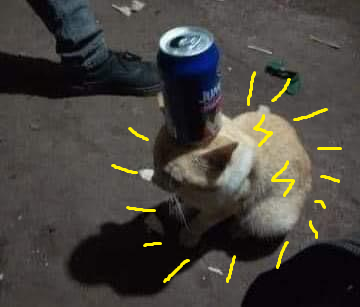
\includegraphics[width=0.5\linewidth]{el.png}
    \caption{Electrogato}
    \label{fig:enter-label}
\end{figure}\\

\begin{thebibliography}{99}

\bibitem{griffiths}
D. J. Griffiths, \textit{Introduction to Electrodynamics}, 3rd ed. Upper Saddle River, NJ, USA: Prentice-Hall, 1999.

\bibitem{jackson}
J. D. Jackson, \textit{Classical Electrodynamics}, 3rd ed. New York, NY, USA: Wiley, 1998.

\bibitem{sadiku}
M. N. O. Sadiku, \textit{Elements of Electromagnetics}, 6th ed. New York, NY, USA: Oxford University Press, 2014.

\bibitem{wangsness}
R. K. Wangsness, \textit{Electromagnetic Fields}, 2nd ed. New York, NY, USA: Wiley, 1986.

\bibitem{zangwill}
A. Zangwill, \textit{Modern Electrodynamics}. Cambridge, UK: Cambridge University Press, 2013.

\bibitem{purcell}
E. M. Purcell and D. J. Morin, \textit{Electricity and Magnetism}, 3rd ed. Cambridge, UK: Cambridge University Press, 2013.

\bibitem{shadowitz}
A. Shadowitz, \textit{The Electromagnetic Field}. Mineola, NY, USA: Dover Publications, 1988.

\bibitem{Feynman}
Feynman, R. P.  \textit{Lectures on physics}. Addison-Wesley. 1964.

\end{thebibliography}


\end{document}